% Options for packages loaded elsewhere
% Options for packages loaded elsewhere
\PassOptionsToPackage{unicode}{hyperref}
\PassOptionsToPackage{hyphens}{url}
\PassOptionsToPackage{dvipsnames,svgnames,x11names}{xcolor}
%
\documentclass[
  letterpaper,
  DIV=11,
  numbers=noendperiod]{scrreprt}
\usepackage{xcolor}
\usepackage{amsmath,amssymb}
\setcounter{secnumdepth}{5}
\usepackage{iftex}
\ifPDFTeX
  \usepackage[T1]{fontenc}
  \usepackage[utf8]{inputenc}
  \usepackage{textcomp} % provide euro and other symbols
\else % if luatex or xetex
  \usepackage{unicode-math} % this also loads fontspec
  \defaultfontfeatures{Scale=MatchLowercase}
  \defaultfontfeatures[\rmfamily]{Ligatures=TeX,Scale=1}
\fi
\usepackage{lmodern}
\ifPDFTeX\else
  % xetex/luatex font selection
\fi
% Use upquote if available, for straight quotes in verbatim environments
\IfFileExists{upquote.sty}{\usepackage{upquote}}{}
\IfFileExists{microtype.sty}{% use microtype if available
  \usepackage[]{microtype}
  \UseMicrotypeSet[protrusion]{basicmath} % disable protrusion for tt fonts
}{}
\makeatletter
\@ifundefined{KOMAClassName}{% if non-KOMA class
  \IfFileExists{parskip.sty}{%
    \usepackage{parskip}
  }{% else
    \setlength{\parindent}{0pt}
    \setlength{\parskip}{6pt plus 2pt minus 1pt}}
}{% if KOMA class
  \KOMAoptions{parskip=half}}
\makeatother
% Make \paragraph and \subparagraph free-standing
\makeatletter
\ifx\paragraph\undefined\else
  \let\oldparagraph\paragraph
  \renewcommand{\paragraph}{
    \@ifstar
      \xxxParagraphStar
      \xxxParagraphNoStar
  }
  \newcommand{\xxxParagraphStar}[1]{\oldparagraph*{#1}\mbox{}}
  \newcommand{\xxxParagraphNoStar}[1]{\oldparagraph{#1}\mbox{}}
\fi
\ifx\subparagraph\undefined\else
  \let\oldsubparagraph\subparagraph
  \renewcommand{\subparagraph}{
    \@ifstar
      \xxxSubParagraphStar
      \xxxSubParagraphNoStar
  }
  \newcommand{\xxxSubParagraphStar}[1]{\oldsubparagraph*{#1}\mbox{}}
  \newcommand{\xxxSubParagraphNoStar}[1]{\oldsubparagraph{#1}\mbox{}}
\fi
\makeatother


\usepackage{longtable,booktabs,array}
\newcounter{none} % for unnumbered tables
\usepackage{calc} % for calculating minipage widths
% Correct order of tables after \paragraph or \subparagraph
\usepackage{etoolbox}
\makeatletter
\patchcmd\longtable{\par}{\if@noskipsec\mbox{}\fi\par}{}{}
\makeatother
% Allow footnotes in longtable head/foot
\IfFileExists{footnotehyper.sty}{\usepackage{footnotehyper}}{\usepackage{footnote}}
\makesavenoteenv{longtable}
\usepackage{graphicx}
\makeatletter
\newsavebox\pandoc@box
\newcommand*\pandocbounded[1]{% scales image to fit in text height/width
  \sbox\pandoc@box{#1}%
  \Gscale@div\@tempa{\textheight}{\dimexpr\ht\pandoc@box+\dp\pandoc@box\relax}%
  \Gscale@div\@tempb{\linewidth}{\wd\pandoc@box}%
  \ifdim\@tempb\p@<\@tempa\p@\let\@tempa\@tempb\fi% select the smaller of both
  \ifdim\@tempa\p@<\p@\scalebox{\@tempa}{\usebox\pandoc@box}%
  \else\usebox{\pandoc@box}%
  \fi%
}
% Set default figure placement to htbp
\def\fps@figure{htbp}
\makeatother





\setlength{\emergencystretch}{3em} % prevent overfull lines

\providecommand{\tightlist}{%
  \setlength{\itemsep}{0pt}\setlength{\parskip}{0pt}}



 


\KOMAoption{captions}{tableheading}
\makeatletter
\@ifpackageloaded{bookmark}{}{\usepackage{bookmark}}
\makeatother
\makeatletter
\@ifpackageloaded{caption}{}{\usepackage{caption}}
\AtBeginDocument{%
\ifdefined\contentsname
  \renewcommand*\contentsname{Table of contents}
\else
  \newcommand\contentsname{Table of contents}
\fi
\ifdefined\listfigurename
  \renewcommand*\listfigurename{List of Figures}
\else
  \newcommand\listfigurename{List of Figures}
\fi
\ifdefined\listtablename
  \renewcommand*\listtablename{List of Tables}
\else
  \newcommand\listtablename{List of Tables}
\fi
\ifdefined\figurename
  \renewcommand*\figurename{Figure}
\else
  \newcommand\figurename{Figure}
\fi
\ifdefined\tablename
  \renewcommand*\tablename{Table}
\else
  \newcommand\tablename{Table}
\fi
}
\@ifpackageloaded{float}{}{\usepackage{float}}
\floatstyle{ruled}
\@ifundefined{c@chapter}{\newfloat{codelisting}{h}{lop}}{\newfloat{codelisting}{h}{lop}[chapter]}
\floatname{codelisting}{Listing}
\newcommand*\listoflistings{\listof{codelisting}{List of Listings}}
\makeatother
\makeatletter
\makeatother
\makeatletter
\@ifpackageloaded{caption}{}{\usepackage{caption}}
\@ifpackageloaded{subcaption}{}{\usepackage{subcaption}}
\makeatother
\usepackage{bookmark}
\IfFileExists{xurl.sty}{\usepackage{xurl}}{} % add URL line breaks if available
\urlstyle{same}
\hypersetup{
  pdftitle={Den långa bluffen},
  pdfauthor={Christian Lindell \& Alex Voronov},
  colorlinks=true,
  linkcolor={blue},
  filecolor={Maroon},
  citecolor={Blue},
  urlcolor={Blue},
  pdfcreator={LaTeX via pandoc}}


\title{Den långa bluffen}
\author{Christian Lindell \& Alex Voronov}
\date{2026-02-23}
\begin{document}
\maketitle

\renewcommand*\contentsname{Table of contents}
{
\setcounter{tocdepth}{2}
\tableofcontents
}

\bookmarksetup{startatroot}

\chapter*{Förord från boken ``Den långa bluffen - Myterna om Sverige,
arbete och
invandring''}\label{fuxf6rord-fruxe5n-boken-den-luxe5nga-bluffen---myterna-om-sverige-arbete-och-invandring}
\addcontentsline{toc}{chapter}{Förord från boken ``Den långa bluffen -
Myterna om Sverige, arbete och invandring''}

\markboth{Förord från boken ``Den långa bluffen - Myterna om Sverige,
arbete och invandring''}{Förord från boken ``Den långa bluffen - Myterna
om Sverige, arbete och invandring''}

\href{https://volante.se/bocker/den-langa-bluffen/}{\begin{center}
\pandocbounded{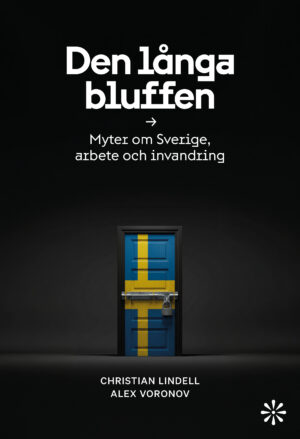
\includegraphics[keepaspectratio]{bilder/Den-langa-bluffen-Framsida-300x439.jpg}}
\end{center}
}

En lång bluff i poker är en bluffstrategi där en spelare har en svag
hand men spelar på ett sätt som får motspelarna att tro motsatsen. De
felaktiga föreställningarna byggs upp under lång tid, över flera
satsningsomgångar.

En bluff kan även vara lång i betydelsen långlivad. Den kan ha formen av
en villfarelse som håller sig länge i det allmänna medvetandet.

Diskussionen om invandring, utanförskap och bidrag har haft den här
karaktären under lång tid.

Sverige arbetar som aldrig förr. Bidragsberoendet är det lägsta på 50
år. Flyktingar får jobb allt snabbare. Stora förbättringar har skett
framför allt under det senaste årtiondet.

Men i debatten låter det ofta annorlunda. Påståenden om att
utanförskapet är stort, dyrt och växande och att integrationen har
misslyckats, yttras inte bara som slentrianpladder på diverse nätforum.
De uttrycks dagligen av ledande politiker och tar sig in i partiprogram,
statliga policydokument och lägger grund för lagstiftning.

De leder till vanföreställningar och fördomar, och blir argument för en
politik som stänger gränser, skapar klyftor, skadar människor och gör
Sverige till ett sämre land än det borde vara.

Vi vill bidra till att förändra detta. Syftet med boken är att spräcka
en rad myter om invandring och ekonomi, men även om tillståndet på
arbetsmarknaden i allmänhet.

En myt är att Sverige har stora problem med arbetslöshet och att läget
var bättre förr. En annan myt är att invandrare har allt svårare att
etablera sig i vårt land. Besläktade myter är att det ekonomiska läget i
utsatta områden förvärras och att det stora flyktingmottagandet för tio
år sedan blev ett sänke i kommunerna.

Var gränsen för asylsökande verkligen nådd 2015? Hur står det till i de
så kallade utanförskapsområdena? Och vad hände egentligen i Filipstad?

Vi tar itu med hittepåbegrepp som självförsörjning och
integrationsskuld. Vi visar hur målen att minska invandringen krockar
med de negativa befolkningssiffrorna och suget efter arbetskraft.

Det gör vi genom statistik som oftast finns tillgänglig för var och en,
men som sällan lyfts fram i diskussionen eller sammanställs till en
helhet.

Vi hoppas att det här kan vara en handbok för den som vill argumentera
mot skrämselpropagandan och behöver pålitliga siffror, källor, relevanta
infallsvinklar och förklaringar.

\emph{Alex Voronov och Christian Lindell, maj 2026}

\bookmarksetup{startatroot}

\chapter{``Sysselsättning'' är samma sak som
``förvärvsarbete''}\label{sysselsuxe4ttning-uxe4r-samma-sak-som-fuxf6rvuxe4rvsarbete}

Det cirkulerar väldigt många okunniga kommentarer om vad
``sysselsättning'' är i arbetsmarknadsstatistiken. Vi tar det från
början: \emph{sysselsättning = förvärvsarbete}. För att vara sysselsatt
måste man få \emph{lön} \emph{från en arbetsgivare} eller \emph{arbeta i
eget eller anhörigs företag}. Det är den definition som SCB använder i
den officiella sysselsättningsstatistiken som kommer från
Arbetskraftsundersökningarna (AKU).

Apokalypshögern brukar älska att citera Ekonomifakta om vad
sysselsättning är:

\pandocbounded{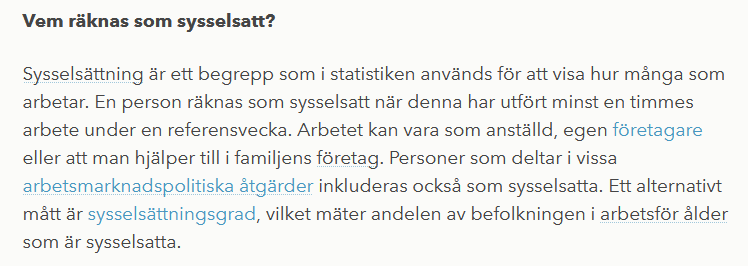
\includegraphics[keepaspectratio]{bilder/vad_ar_sysselsattning/sysselsattning_ekfakta.PNG}}

Ofta åtföljs hänvisningen till Ekonomifakta av påståenden som
``Värdelöst mått! Det räcker att jobba en enda timme!''. ``Man behöver
inte ens få betalt!'', ``Det räcker att man är går på SFI en timme i
veckan så är man sysselsatt!'', ``Det räcker att delta i en
pysselsättning hos Arbetsförmedlingen 1 timme i veckan för att räknas
som sysselsatt!''.

De frågor man \emph{inte} ställer sig är:

\begin{itemize}
\item
  Hur många arbetar så lite som 1 timme i veckan? Är det relevant?
\item
  \emph{Vilka} kan arbeta gratis och räknas som sysselsatta?
\item
  Är SFI och andra utbildningar verkligen ``sysselsättning'' i
  statistiken?
\item
  Vilka är de ``vissa arbetsmarknadspolitiska åtgärder'' som räknas som
  sysselsättning?
\end{itemize}

\emph{Hur stor andel av de sysselsatta klassas som sysselsatta genom att
arbeta väldigt få timmar?}

Det räcker att jobba en timme under mätveckan. Det är sant, men
irrelevant eftersom ingen jobbar så lite (\textless0,2\% av de
sysselsatta). I åldern 20-64 år är det 97\% av de sysselsatta som
arbetar minst 20 h/vecka och 83\% som arbetar minst 35 h. Dessa andelar
är i det närmast identiska för både inrikes- och utrikesfödda.

\emph{Behöver man inte ens ha betalt för att jobba för att räknas som
``sysselsatt''?}

Om man arbetar i ett familjeföretag så antas man få del av avkastningen
utan att man får någon formell lön. Ett typiskt exempel är
lantbruksföretag som av tradition tidigare oftast ägdes av mannen i
familjen. Hustrun var formellt hemmafru, men jobbade större delen av
tiden med lantbruket. Båda två levde på lantbruket, men det var
\emph{formellt} bara mannen som försörjdes av det. Så det stämmer att
man inte behöver få betalt för att räknas som ``sysselsatt'' under
förutsättning av att man arbetar i en anhörigs företag.

\emph{Bidragsjobb då?}

Det är endast de insatser från Arbetsförmedlingen som sker i form av
lönesubvention till arbetsgivare som gör att man räknas som
``sysselsatt''. Då har man \emph{lön} (inte bidrag!) \emph{från en
arbetsgivare,} vilket överensstämmer med definitionen av
``sysselsättning''. Ungefär 35\% av de som deltar i
arbetsmarknadspolitiska åtgärder via Arbetsförmedlingen deltar i sådana
insatser som gör att de räknas som ``sysselsatta''. I absoluta tal
handlar det om ca 80 00 personer, varav 60 \% får stöd pga nedsatt
arbetsförmåga. Stöden höjer sysselsättningsgraden för befolkningen
mellan 16-65 år med drygt 1,2 procentenheter. För gruppen födda utanför
Europa höjs sysselsättningsgraden med drygt 1,8 procentenheter. Ingen
försumbar andel, men heller inte så många att det finns skäl att
ifrågasätta sysselsättningsmåttet.

Ibland ser man påståenden om att deltagande i FAS 3 räknades som
sysselsättning. Det stämmer inte eftersom de inblandade företagen var
\emph{anordnare} (inte arbetsgivare!) som inte betalade någon lön.
Deltagarna ersattes oftast av aktivitetsstöd och i vissa fall av
ekonomiskt bistånd från kommunen. De hade alltså bidrag och inte lön och
uppfyllde därmed inte kriterierna för att räknas som sysselsatta.

Antalet personer som är ``sysselsatta'' via stöd från Af är kraftigt
minskande. Det är inte heller så att det är en höger-vänster-fråga vilka
regeringar som satsar på subventionerade tjänster.

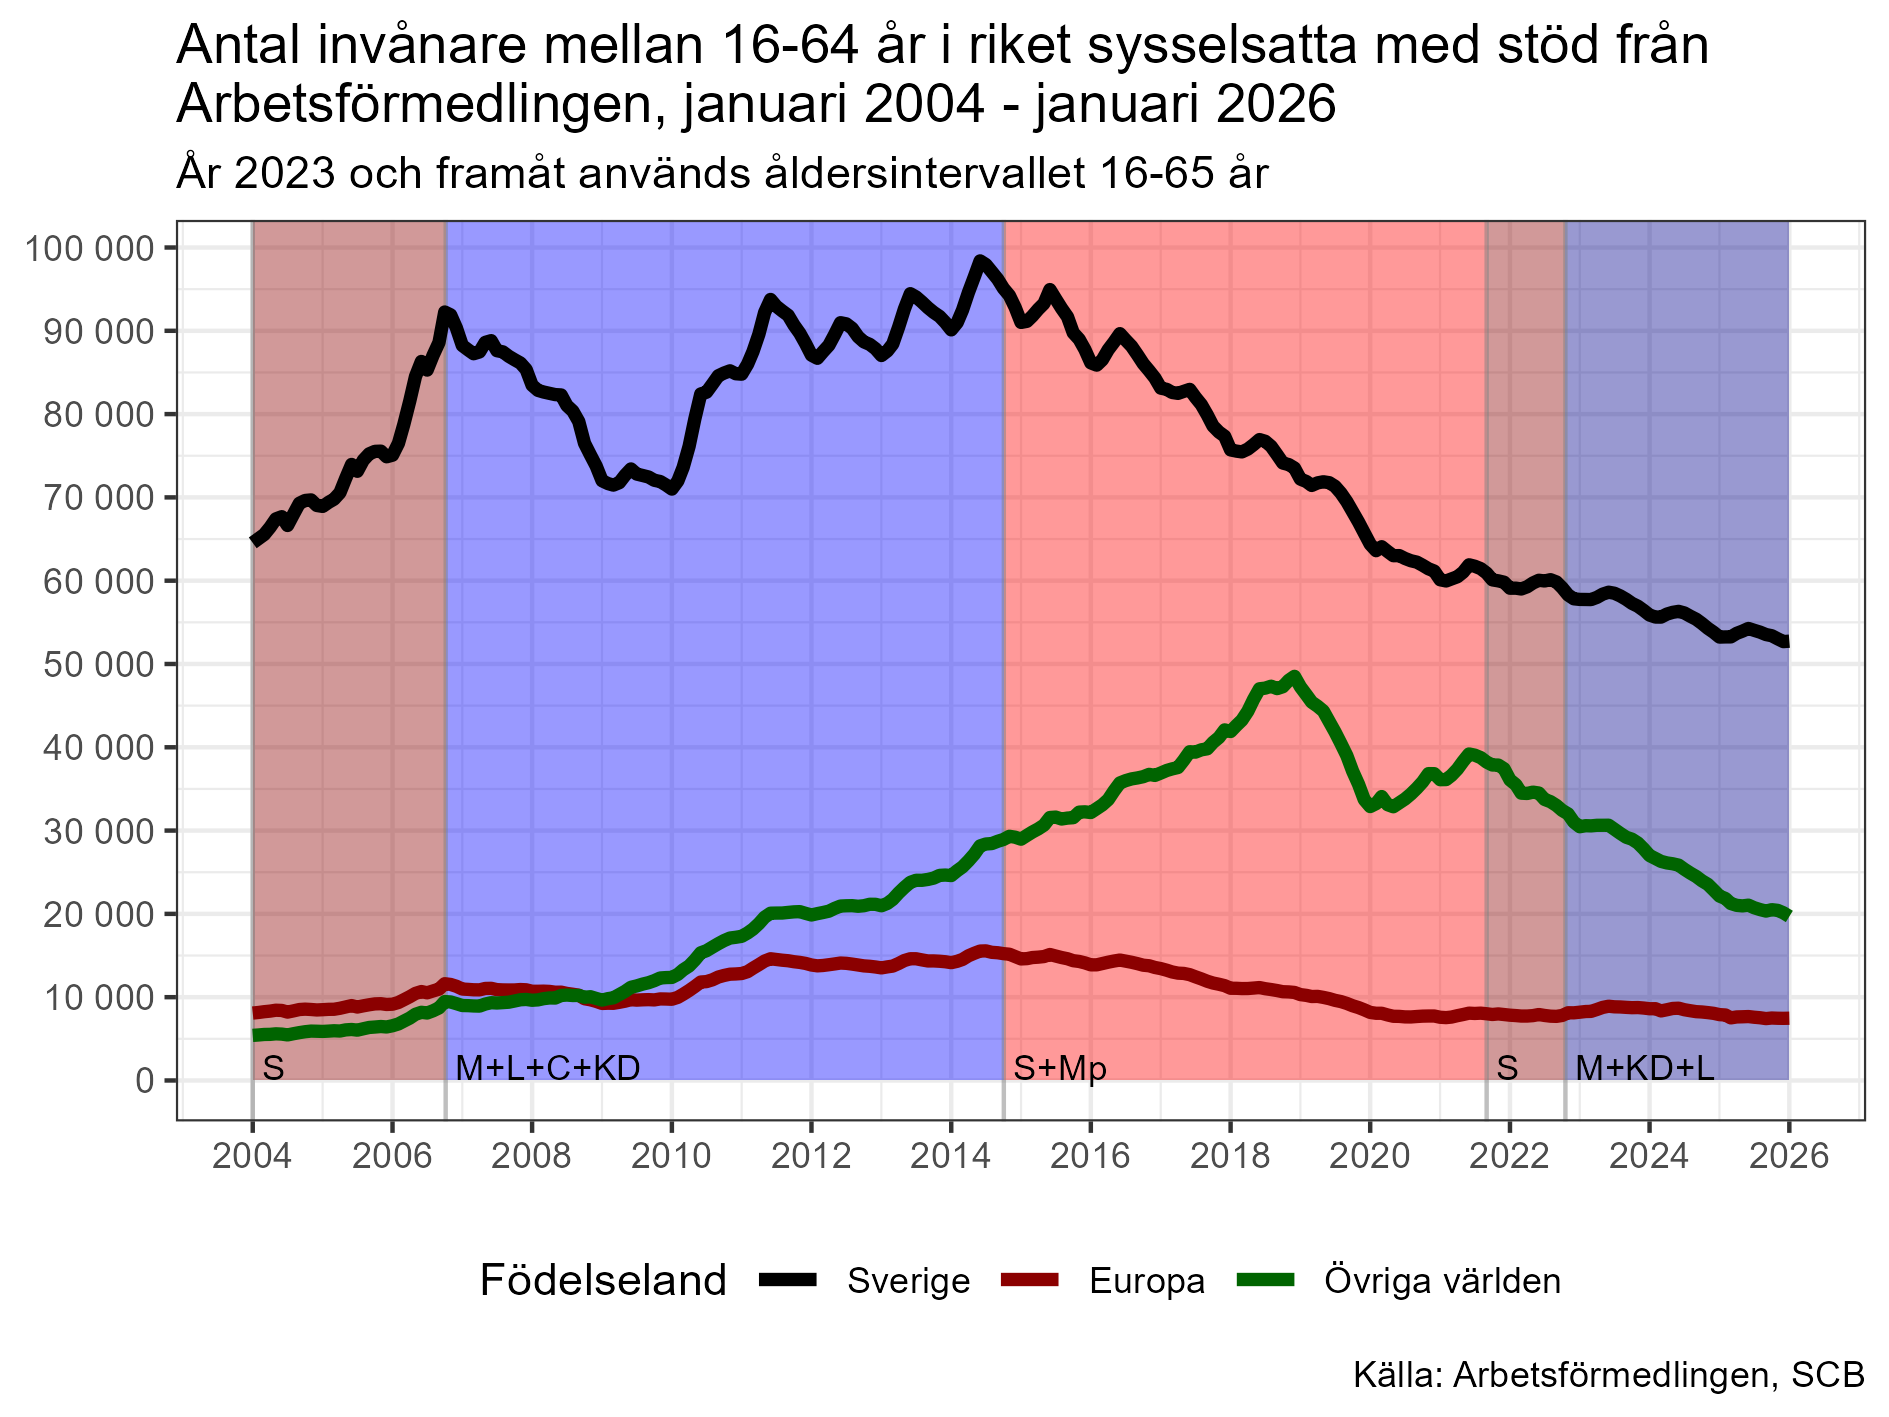
\includegraphics[width=16cm,height=\textheight,keepaspectratio]{bilder/vad_ar_sysselsattning/dia_bakgrund_reg_abs.png}

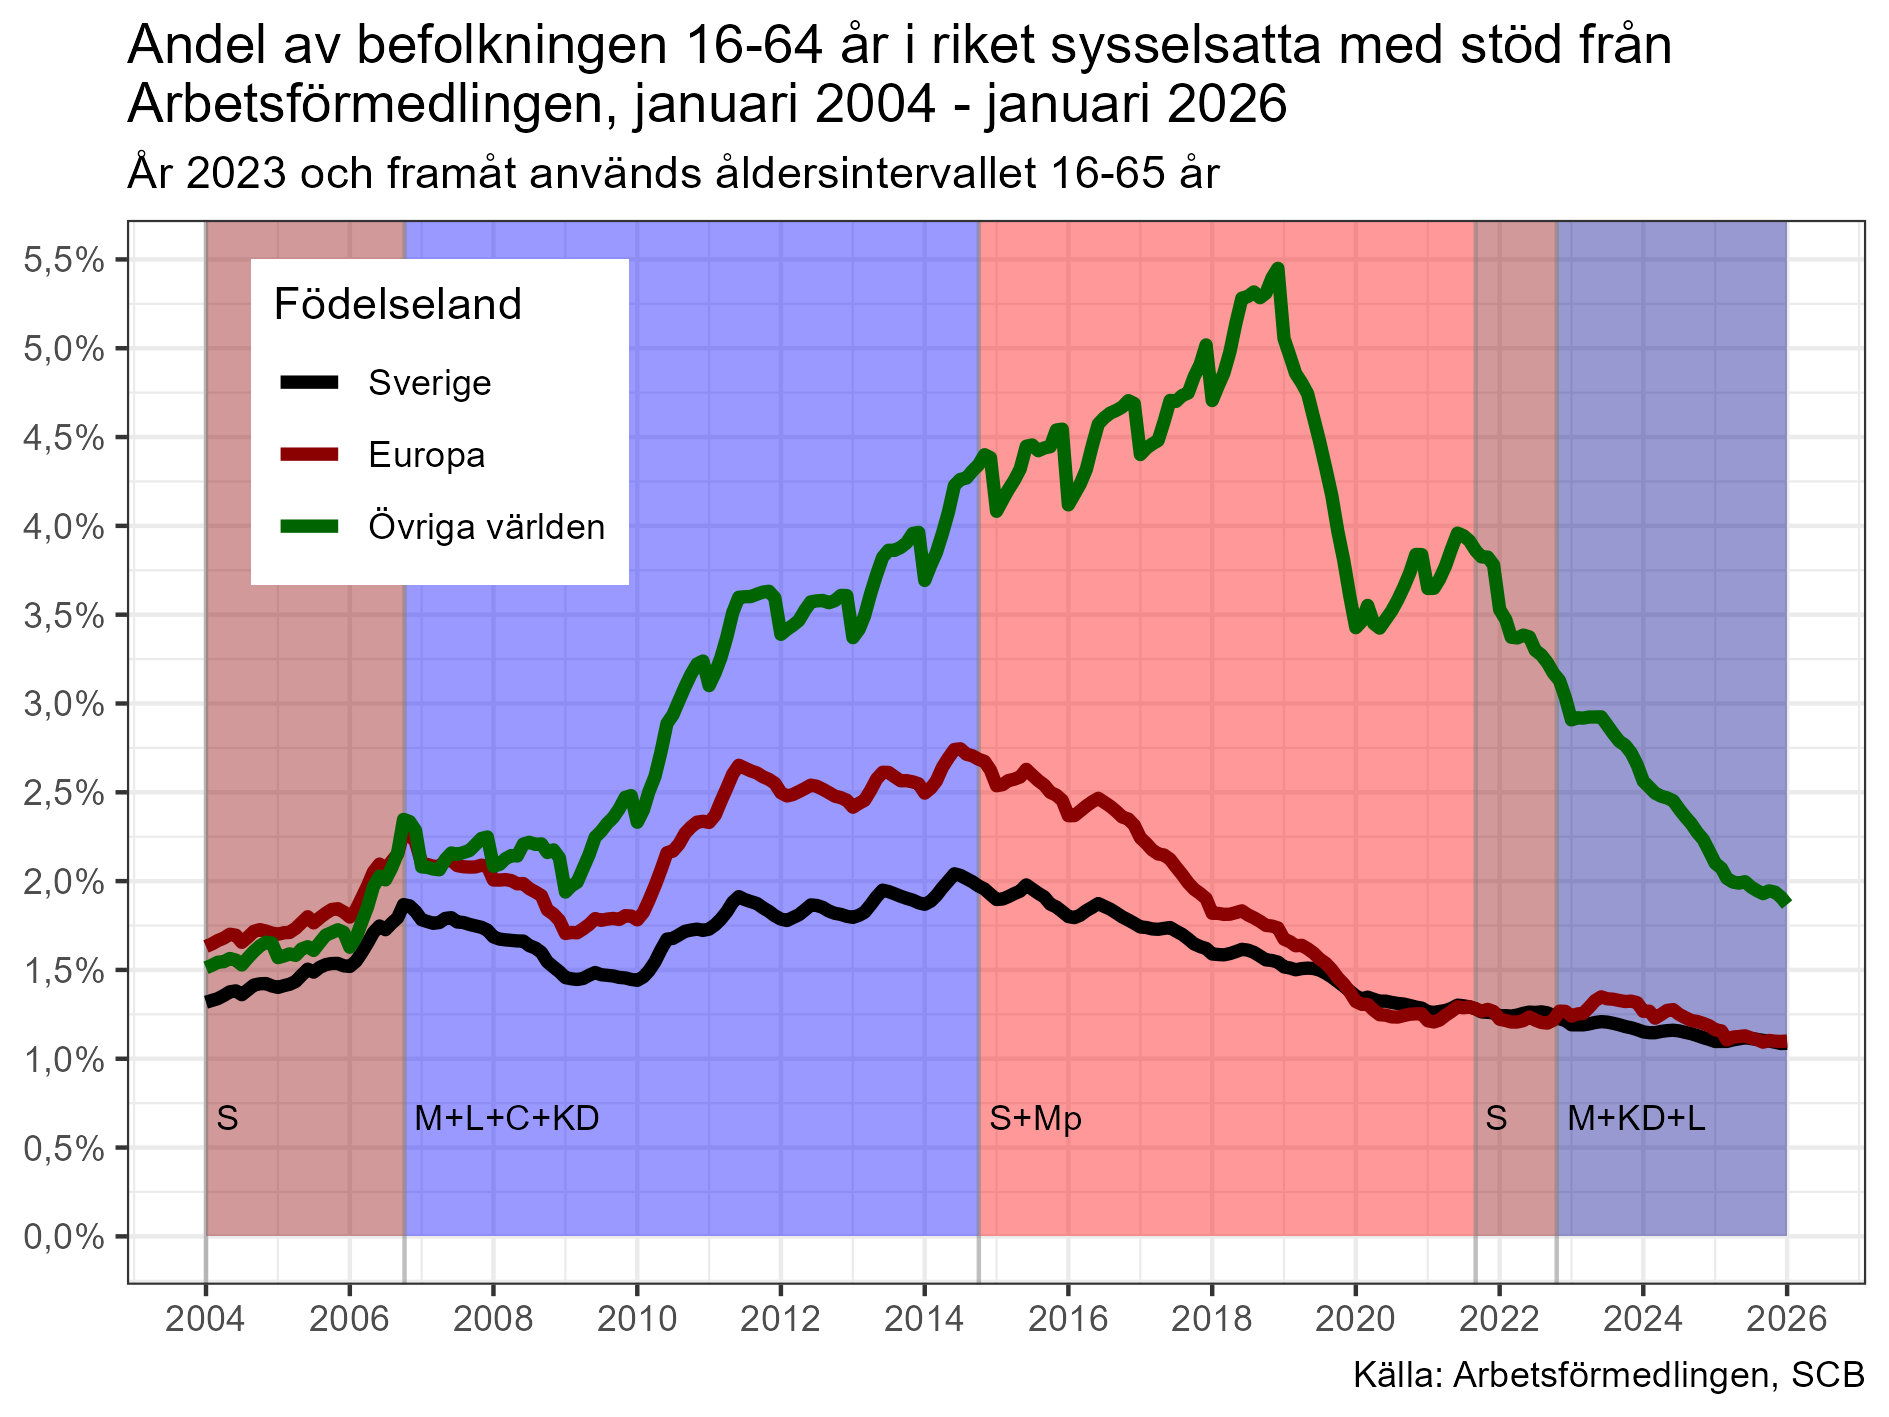
\includegraphics[width=16cm,height=\textheight,keepaspectratio]{bilder/vad_ar_sysselsattning/dia_bakgrund_reg_pct.png}

\emph{Räcker det att läsa SFI för att räknas som ``sysselsatt''?}

Nej. Det är entydigt fel. Om man läser SFI är man inte ``sysselsatt''
eftersom det inte finns någon arbetsgivare. Om man läser en utbildning
är man just i kategorin ``Utbildning''. Man är inte ``sysselsatt'',
såvida man inte arbetar vid sidan om studierna.

\emph{Håller regeringen på att manipulera statistiken?}

Man läser ibland påståenden om att regeringen ändrar definitioner och
manipulerar statistiken. Det stämmer inte heller. Definitionerna inom
arbetsmarknadsstatistiken regleras i en
\href{https://www.ilo.org/resource/resolution-concerning-statistics-work-employment-and-labour}{ILO-resolution}
som alla länder följer. Senaste upplagan är från 2023. Dessa
definitioner preciseras ytterligare av EU:s statistikmyndighet Eurostat
som säkrar att arbetsmarknadsstatistiken inom EU är jämförbar.

I ILO:s resolution kan man bland annat se att 1-timmesgränsen är en
internationell standard och man kan se att de som får bidrag (inte lön!)
från Arbetsförmedlingen inte räknas som ``sysselsatta''.

Man läser ibland att ``sossarna'' har hittat på ``sysselsättning'' som
om det vore ett nytt begrepp. Det är naturligtvis inte heller sant. SCB
har mätt ``sysselsättning'' med ungefär samma definition i alla fall i
50 år. Det finns tidsserier sedan 1970 i SCB:s öppna databas. (Jag har
läst påstående om att mätningarna började redan 1960, men jag har inte
kunnat verifiera det.)

\emph{Sysselsättning borde heta förvärvsarbete!}

En sak som stör mig är att SCB valt att tala om ``sysselsatta'' och inte
``förvärvsarbetande''. Det hade minskat förvirringen runt
sysselsättningsbegreppet som inte har samma betydelse i vardagsspråket
som det har som statistiskt begrepp. På engelska heter det
``employment''.

\emph{Tänk lite själva!}

Och tänk lite innan ni vidarebefordrar konstiga påstående. Om något
låter för dumt för att vara sant så är det oftast inte det. En typiskt
sådant sak är alla tweets om entimmesgränsen. Tänk efter själva: Är det
rimligt att den skulle ha någon avgörande betydelse? Hur många känner ni
som jobbar 1 timme i veckan? Är det rimligt att en arbetsgivare skulle
lägga ner handläggningstid för att få bidrag för det?

\textbf{KÄLLOR:}

Definition av arbetsmarknadsstatistiken i AKU:

\url{https://www.scb.se/contentassets/8ab23deb3310477a9dad083750ec0355/begrepp-och-definitioner-aku-2021-02-22.pdf}

Få sysselsatta arbetar få timmar:
\url{https://scb.se/hitta-statistik/artiklar/2017/Vanligast-att-unga-och-aldre-jobbar-fa-timmar/}

Ingen skillnad i jobbade timmar mellan sysselsatta inrikesfödda och
flyktingar:
\url{https://www.scb.se/hitta-statistik/artiklar/2019/genomsnittlig-arbetstid-densamma-for-flyktingar-som-for-inrikes-fodda/}

Väldigt få har en överenskommen arbetstid på under 20 h / vecka: Till
exempel Tab2 i någon av tabellerna som heter
``grundtabeller\_månad\_år.xlsx'':

\url{https://www.scb.se/hitta-statistik/statistik-efter-amne/arbetsmarknad/arbetskraftsundersokningar/arbetskraftsundersokningarna-aku/pong/tabell-och-diagram/icke-sasongrensade-data/grundtabeller-aku-1574-ar-manad/}

Sysselsatta i arbetsmarknadspolitiska åtgärder som innebär
lönesubvention till arbetsgivare. se tabellen som heter ``Arbetssökande
1996--årtal-månad'':
\url{https://arbetsformedlingen.se/statistik/sok-statistik/tidigare-statistik}

Allmän statistik om Arbetskraftsundersökningarna hittar man på
\url{http://scb.se/aku} .

Jämförelser med andra EU-länder hittar man på Eurostat:
\url{https://ec.europa.eu/eurostat/data/database} Leta under:

\pandocbounded{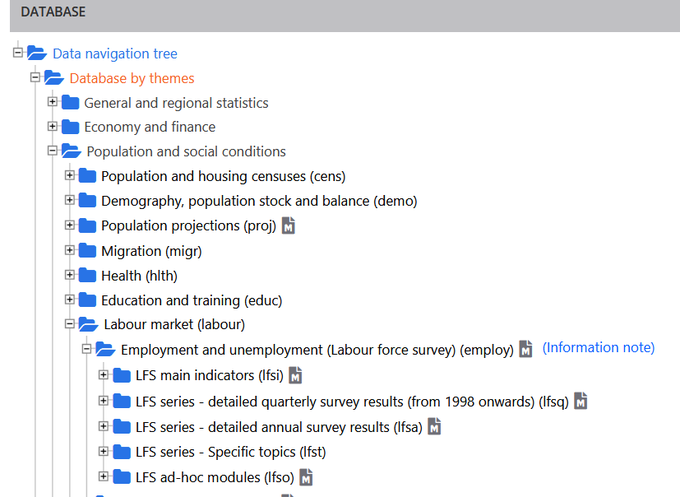
\includegraphics[keepaspectratio]{bilder/vad_ar_sysselsattning/eurostat.png}}

Löpande månadsstatistik från Af hittar man här:
\url{https://arbetsformedlingen.se/statistik/sok-statistik}

\bookmarksetup{startatroot}

\chapter{Det går snabbare för flyktingar att få
jobb}\label{det-guxe5r-snabbare-fuxf6r-flyktingar-att-fuxe5-jobb}

Runt 2010 skedde ett skifte i hur många år det tar för flyktingar och
anhöriga att få arbete. Det finns en tydlig trend som visar att det går
allt snabbare för flyktingar att få jobb. Kanske är det därför det finns
ett antal studier som räknar medelvärde för tid till arbete som bygger
på medelvärde från 1990 och framåt. Då kan man nämligen undvika att visa
att det finns en trend i statistiken som visar att tiden blir allt
kortare.

Diagrammet nedan visar tid in till arbete efter vilket år flyktingarna
blivit kommunplacerade. De som kommunplacerarades mellan åren 2000-2024
tog det nio år innan hälften var sysselsatta. För de som
kommunplacerades 2020 tog det mindre än tre år.

\pandocbounded{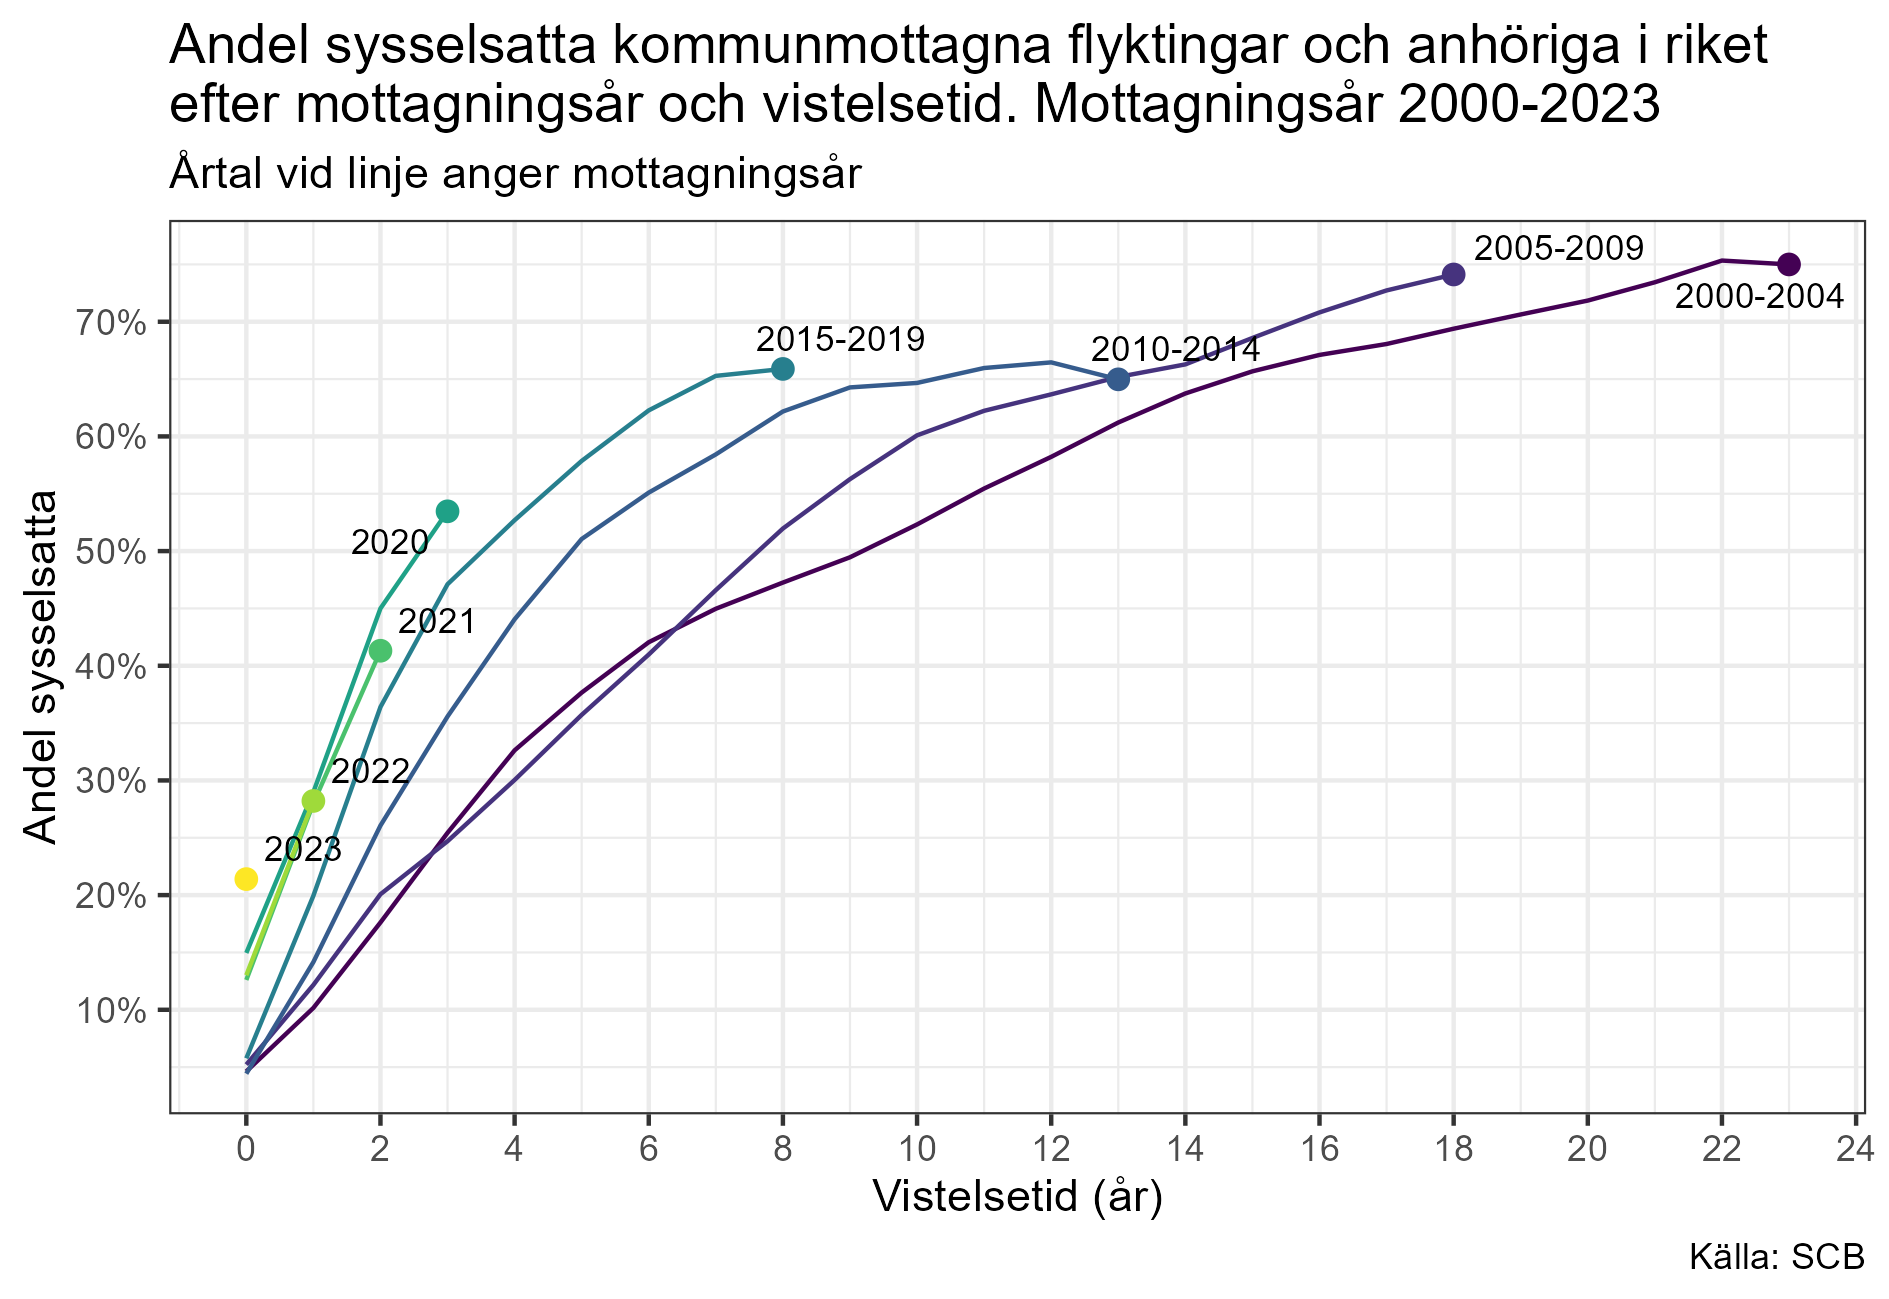
\includegraphics[keepaspectratio]{bilder/flyktingar_vt/flyktingar_sysgrad_vistelsetid_Riket.png}}

Men det är stora skillnader mellan män och kvinnor. Män får arbete
betydligt snabbare. På lång sikt utjämnas dock skillnaderna. Kvinnor som
kommunplacerades mellan 2000-2009 har i stort sett samma
sysselsättningsgrad som män som kom under samma period.

\pandocbounded{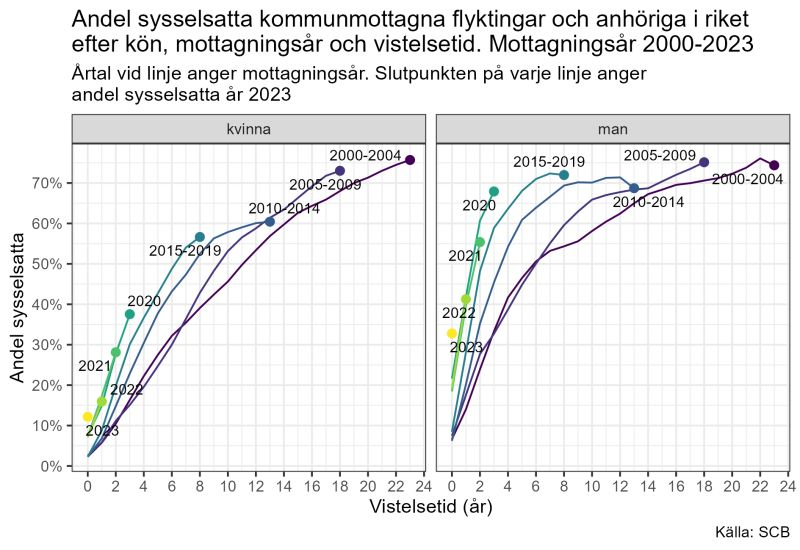
\includegraphics[keepaspectratio]{bilder/flyktingar_vt/flyktingar_vt_kon.jpg}}

Källa:

\href{https://www.statistikdatabasen.scb.se/pxweb/sv/ssd/START__AA__AA0003__AA0003B/MotFlyktLanBAS/}{Andel
sysselsatta kommunmottagna flyktingar och anhöriga efter län, kön,
mottagningsår och sysselsättningsår 2022 - 2023}

\href{https://www.statistikdatabasen.scb.se/pxweb/sv/ssd/START__AA__AA0003__AA0003B/KomMotForvBAS/}{Antal
sysselsatta kommunmottagna flyktingar och anhöriga efter antal år efter
mottagning, kön och mottagningsår 1997 - 2024}

\bookmarksetup{startatroot}

\chapter{Situationen förbättras för utsatta
områdem}\label{situationen-fuxf6rbuxe4ttras-fuxf6r-utsatta-omruxe5dem}

Många som gör sin röst hörd i den offentliga debatten tycks ha missat
utvecklingen i de så kallade utsatta områdena. Det är en av de mest
seglivade myterna att det skulle vara en växande och allt mer
problematisk grupp av områden där människor lever i utanförskap,
kriminalitet och bidragsberoende. Men faktum är att
arbetsmarknadssituationen har förbättrats avsevärt över tid.

Till att börja med har sysselsättningsgraden ökat kraftigt i stadsdelar
med låg sysselsättningsgrad. Vi använder oss här av SCB:s indelning av
Sverige i Regionala StatistikOmråden (som i stort motsvarar stadsdelar
när vi kommer in i städer).

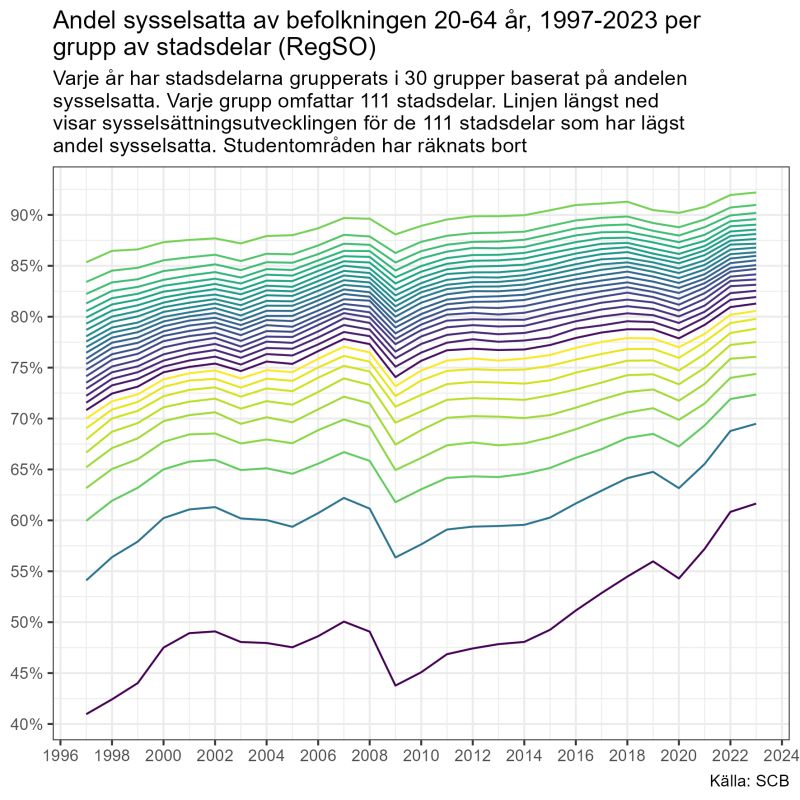
\includegraphics[width=5.98958in,height=\textheight,keepaspectratio]{bilder/regso_utsatta_omr/regso_sysselsattning.jpg}

Den trettiondel av RegSO-områdena som 1997 hade lägst
sysselsättningsgrad arbetade 41 procent av invånarna. 2023 hade andelen
stigit till 59 procent. Sysselsättningsgraden är fortfarande låg, men
tillväxttakten är dramatiskt. Andelen sysselsatta har framför allt ökat
sedan 2010 -- vilket intressant nog sammanfaller med den stora ökningen
av flyktinginvandringen.

Det är sant att det är många osäkra anställningar som ökat och att
lönenivåerna är låga, men även självförsörjningsgrade, det mått som
tidöregeringen ålagt SCB att mäta, visar på en stigande andel
``självförsörjande'' i de områden som har lägst självförsörjningsgrad.
2013 uppgick självförsörjningsgraden till 39 procent av befolkningen
mellan 20-64 i den 30-del av RegSO-områdena som hade lägst
självförsörjningsgrad.

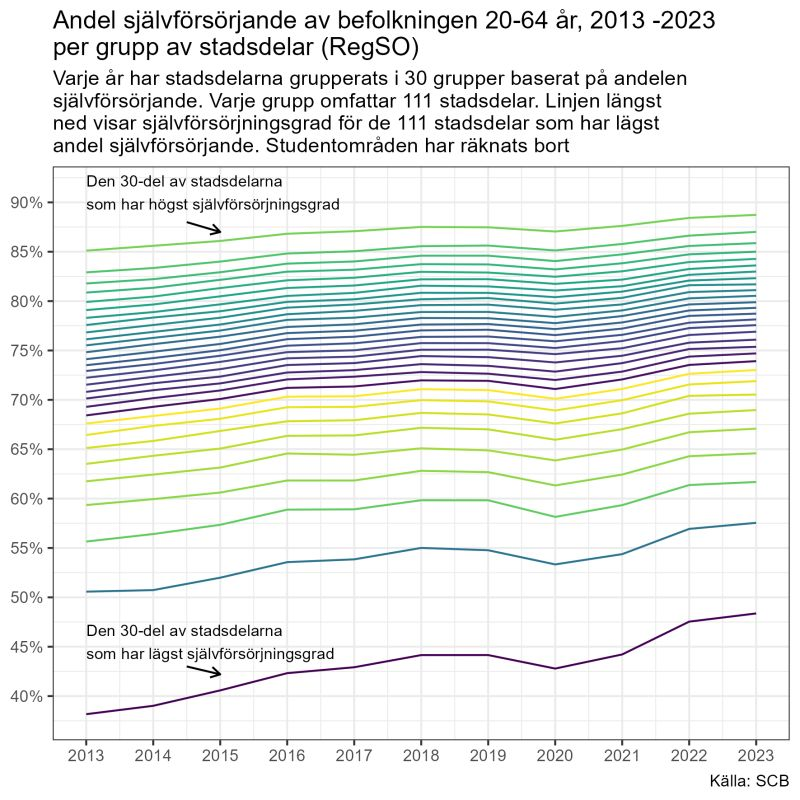
\includegraphics[width=6.13542in,height=\textheight,keepaspectratio]{bilder/regso_utsatta_omr/regso_sjalvforsorjning.jpg}

Ett sista mått vi ska granska är alla politikers favoritmått -- Hur
många barn lever i hushåll där en vuxxen går till jobbet? Det visar sig
att även det måttet ökat kraftigt. 2013 var det 43 procent av barnen
under 18 år som bodde i hushåll där ingen vuxen var registrerad som
sysselsatt i statistiken om vi tittar på den 30-del av RegSO-områdena
som hade högst andel barn i hushåll där ingen arbetar. 2023 hade andelen
minskat till 23 procent.

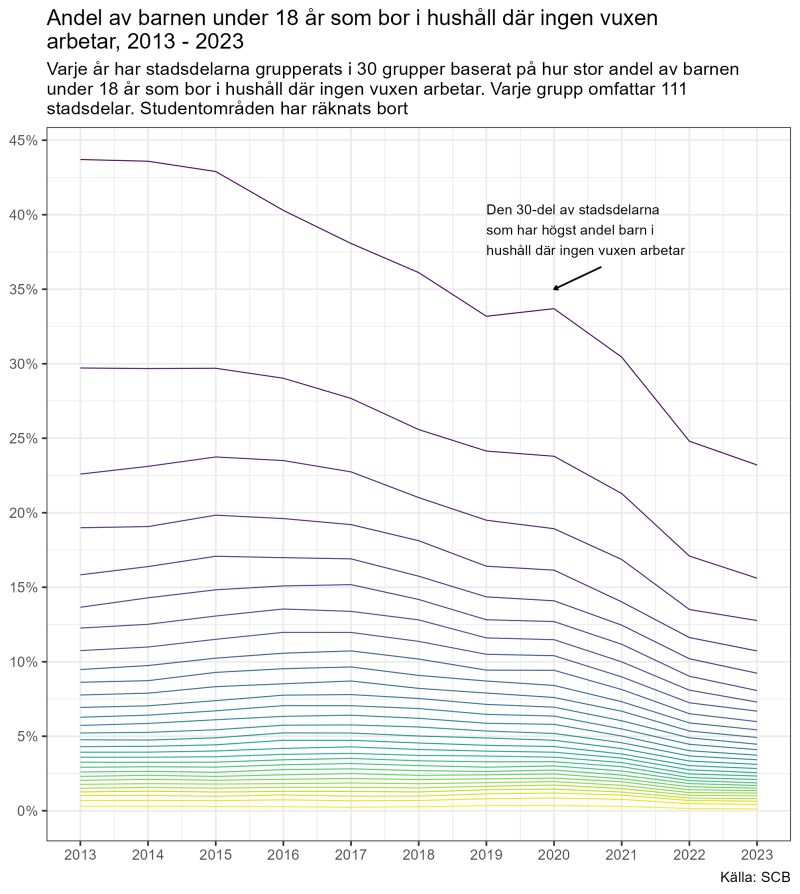
\includegraphics[width=6.21875in,height=\textheight,keepaspectratio]{bilder/regso_utsatta_omr/regso_barn.jpg}

Alla de måtten vi tagit fram visar att det fortfarande finns tydliga
problem i de ofta invandrartäta områden där få arbetar, men att det
samtidigt har blivt markant bättre på relativt kort tid. Diagrammen
speglar den övergripande utvecklingen av att flyktingar kommer in på
arbetsmarknaden allt snabbare, rekordlåga nivåer av befolkningen som
lever på sociala ersättningar och bidrag och stigande
sysselsättningsgrad. Ändå är det märkligt tyst i massmedia om denna
utveckling.

\bookmarksetup{startatroot}

\chapter{Vilken typ av invandrare arbetar i olika
yrken}\label{vilken-typ-av-invandrare-arbetar-i-olika-yrken}

Vilken typ av invandrare dominerar bland invandrartäta yrken?

Ofta drar man i debatten en skarp gräns mellan flykting- och
arbetskraftsinvandring. Men totalt sett har flyktinginvandringen en
större betydelse för arbetskraftsförsörjningen än
arbetskraftsinvandringen från länder utanför EU/EES. Framför allt inom
vård- och omsorg är flyktinginvandringen av stor betydelse. Men även
arbetskraftsinvandringen till vårdyrken är av större betydelse än vad
som ibland framgår av debatten.\\
\strut \\
LO har rätt i att det är liten arbetskraftsinvandring till yrken inom
vård- och omsorg. Men det gäller endast om vi räknar tvärsnitt och ser
till hur många som har arbetstillstånd just nu. Det riskerar att bli
missvisande eftersom många som sökt sig till Sverige som
arbetskraftsinvandrare med tiden rotar sig här och blir svenska
medborgare och inte längre behöver arbetstillstånd.\\
\strut \\
Räknar vi på senast uppgivna grund för bosättning ser vi att det är en
stor grupp som kommit hit som arbetskraftsinvandrare även inom vård- och
omsorg. Många av dessa är numera svenska medborgare och ingår inte
längre i Migrationsverkets statistik över arbetskraftsinvandring.

\pandocbounded{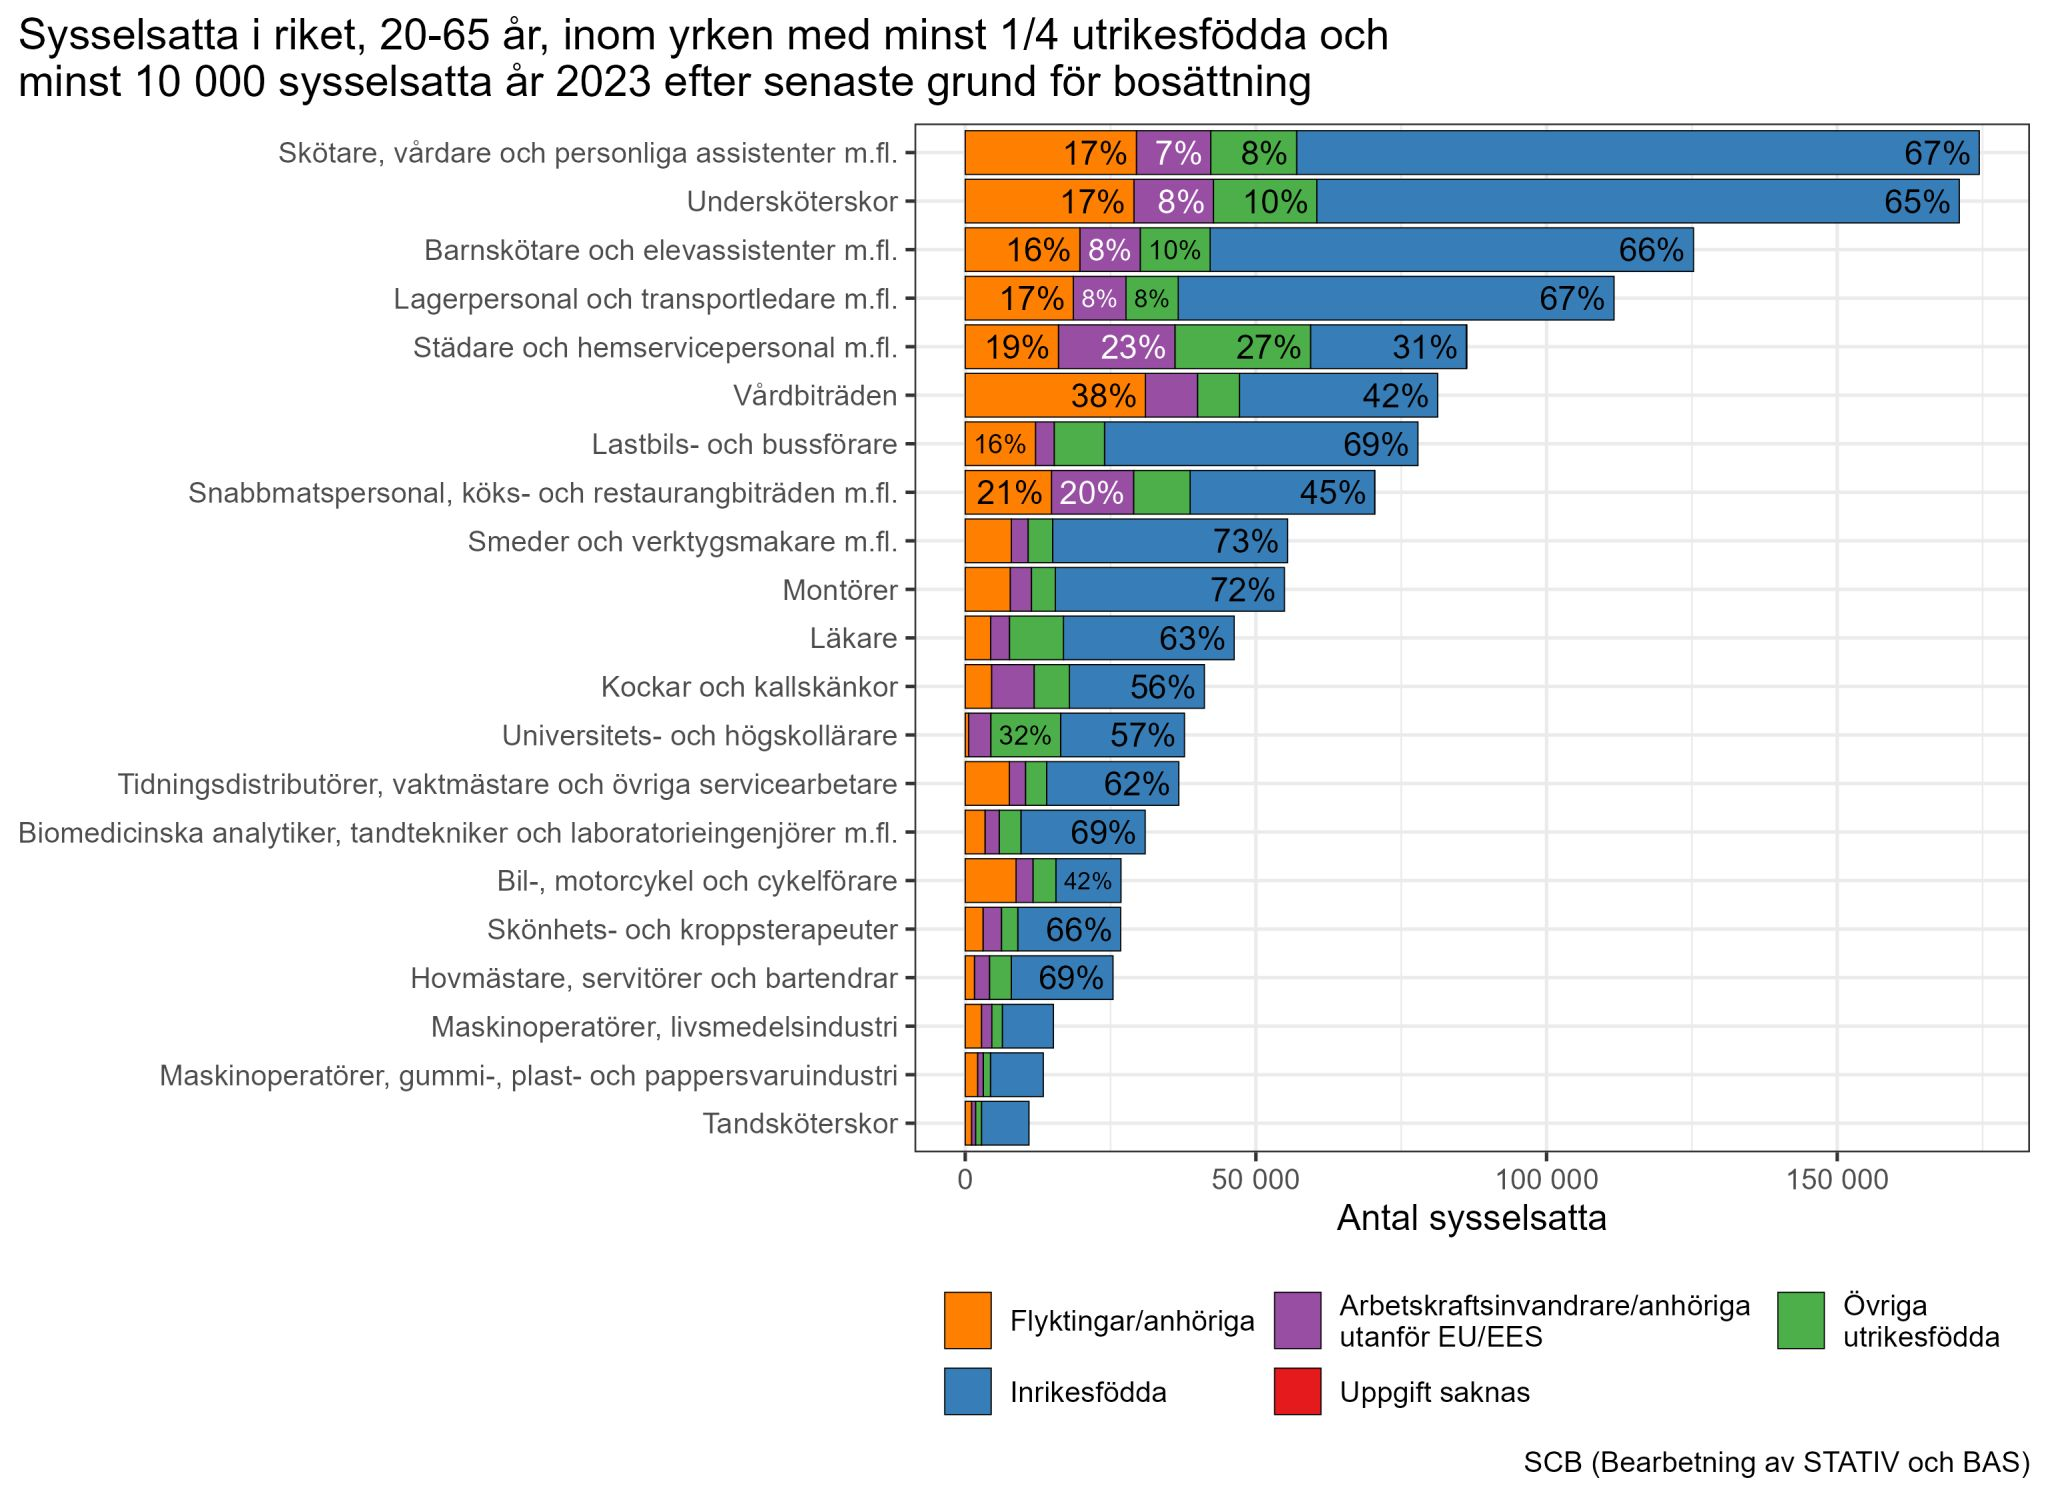
\includegraphics[keepaspectratio]{bilder/gfb_yrken/gfb_yrken.jpg}}

\bookmarksetup{startatroot}

\chapter{Medianålder i Europa och
Sverige}\label{medianuxe5lder-i-europa-och-sverige}

Sverige tillhör de länder som har lägst medianålder i Europa och har,
tillsammans med Malta och Luxemburg, stort sett har oförändrad
medianålder år 2024 jämfört med 2010. Detta är till stor del en följd av
Sveriges stora invandring. Sverige har därmed en betydligt gynnsammare
åldersstruktur än framför allt ett antal länder i sydeuropa.

Italien sticker ut som ett av länderna med högst medelålder. Italien har
dessutom svårt att sysselsätta den förhållandevis lilla andelen av
befolkningen som är i arbetsför ålder och tillhör bottenligan vad gäller
sysselsättningsgrad.

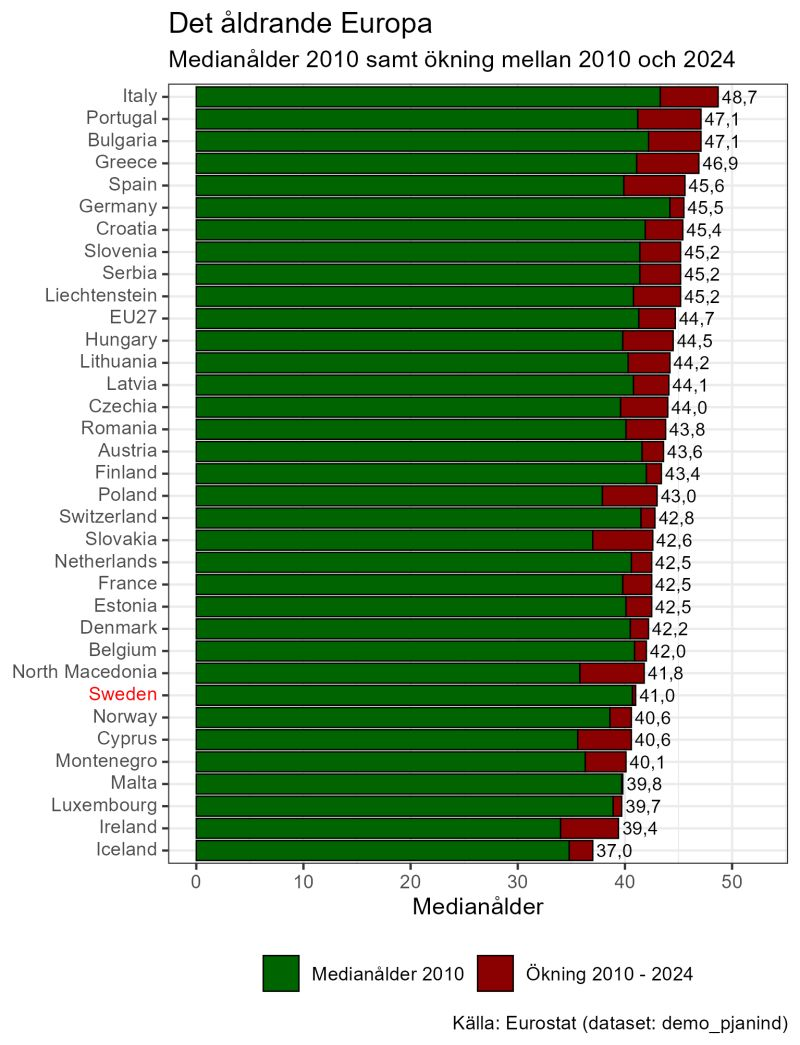
\includegraphics[width=6.82292in,height=\textheight,keepaspectratio]{bilder/demografi_eu/medianalder_EU.jpg}

\bookmarksetup{startatroot}

\chapter{Utrikesfödda möjliggör en ökning av
sysselsättningen}\label{utrikesfuxf6dda-muxf6jligguxf6r-en-uxf6kning-av-sysselsuxe4ttningen}

Utrikesfödda har en betydande roll i att öka sysselsättningen i Sverige.
De bidrar till arbetsmarknaden genom att fylla viktiga funktioner inom
olika sektorer, särskilt inom vård, omsorg och serviceyrken.

2010 var det senaste år då tillväxten av jobb var större bland
inrikesfödda än bland utrikesfödda i absoluta tal. Sedan dess har
utrikesfödda varje år dominerat jobbtillväxten. Samtidigt har andelen
sysselsatta bland utrikesfödda stigit stadigt sedan 2009. År 2016 nådde
sysselsättningsgraden 84 \% för inrikesfödda. Där har den i stort sett
legat kvar med någon enstaka procentenhets variation upp och ned,
oavsett konjunktur och pandemi. Det tycks som om vi nått ett tak för hur
många inrikesfödda som går att sysselsätta. Sedan 2016 domineras
jobbtillväxten fullständigt av utrikesfödda och vi ser till och med en
nettominskning av förvärvsarbetande inrikesfödda: 2024 arbetade det
färre inrikesfödda än det gjorde 2016. Det kan delvis förklaras av att
antalet inrikesfödda i förvärvsarbetande ålder minskat under perioden.

Bortser vi från pandemin kan vi i stort sett se en linjär tillväxt av
sysselsättningsgraden för utrikesfödda från 2009 fram till 2022, från 54
\% till 70 \%. De senaste åren har lågkonjunkturen inneburit en relativt
marginell minskning avsysselsättningsgraden. Om antagandet att vi slagit
i taket för andelen arbetande inrikesfödda stämmer, talar mycket för att
denna utveckling kommer att fortsätta. De senaste årens lågkonjunktur
tycks bara marginellt påverkat sysselsättningen. Enligt SCB:s
preliminära sysselsättningsstatistik (BAS) sjönk sysselsättningsgraden
för utrikesfödda med en halv procentenhet mellan februari 2024 och
februari 2025, men steg sedan med 0,6 procentenheter mellan februari
2025 och februari 2026. Även om det är preliminär statistik så tyder
mycket på att vi för närvarande har den högsta andelen förvärvsarbetande
utriksfödda i arbetsför ålder som uppmätts, i alla fall sedan slutet på
80-talet (vilket vi saknar statistik för).

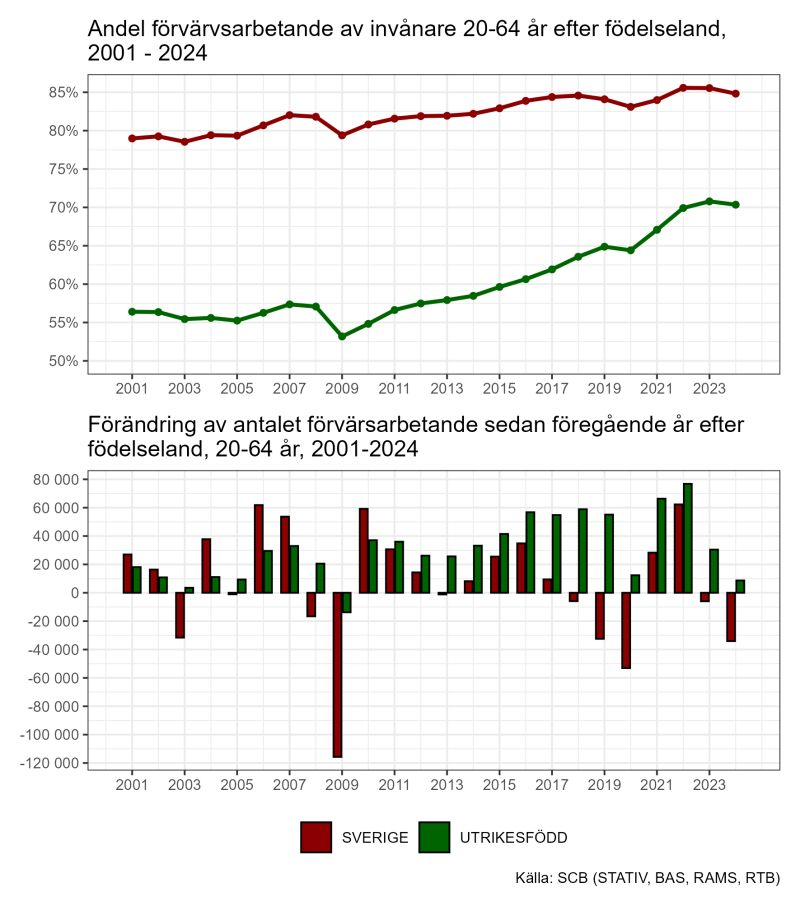
\includegraphics[width=6.29167in,height=\textheight,keepaspectratio]{bilder/sysgrad_fland/sys_fland.jpg}

Två invandrargrupper som drabbats av stormar av hat på sociala medier är
somalier och afghaner. Ofta citeras en gammal artikel från tidningen
Arbetet från 2015 som citerar statistik från 2010 som visar att endast
drygt 20 \% av somalierna i förvärvsarbetande ålder var
förvärvsarbetande. Det stämmer, men som diagrammet nedan visar har
utvecklingen av sysselsättningsgraden varit mycket kraftig sedan dess.
2023 var det 58 \% av somalierna som hade jobb. En nästan lika kraftig
sysselsättningstillväxt ser vi hos afghaner, vars sysselsättningsgrad
stigit från 30 \% 2010 till 70 \% 2023.

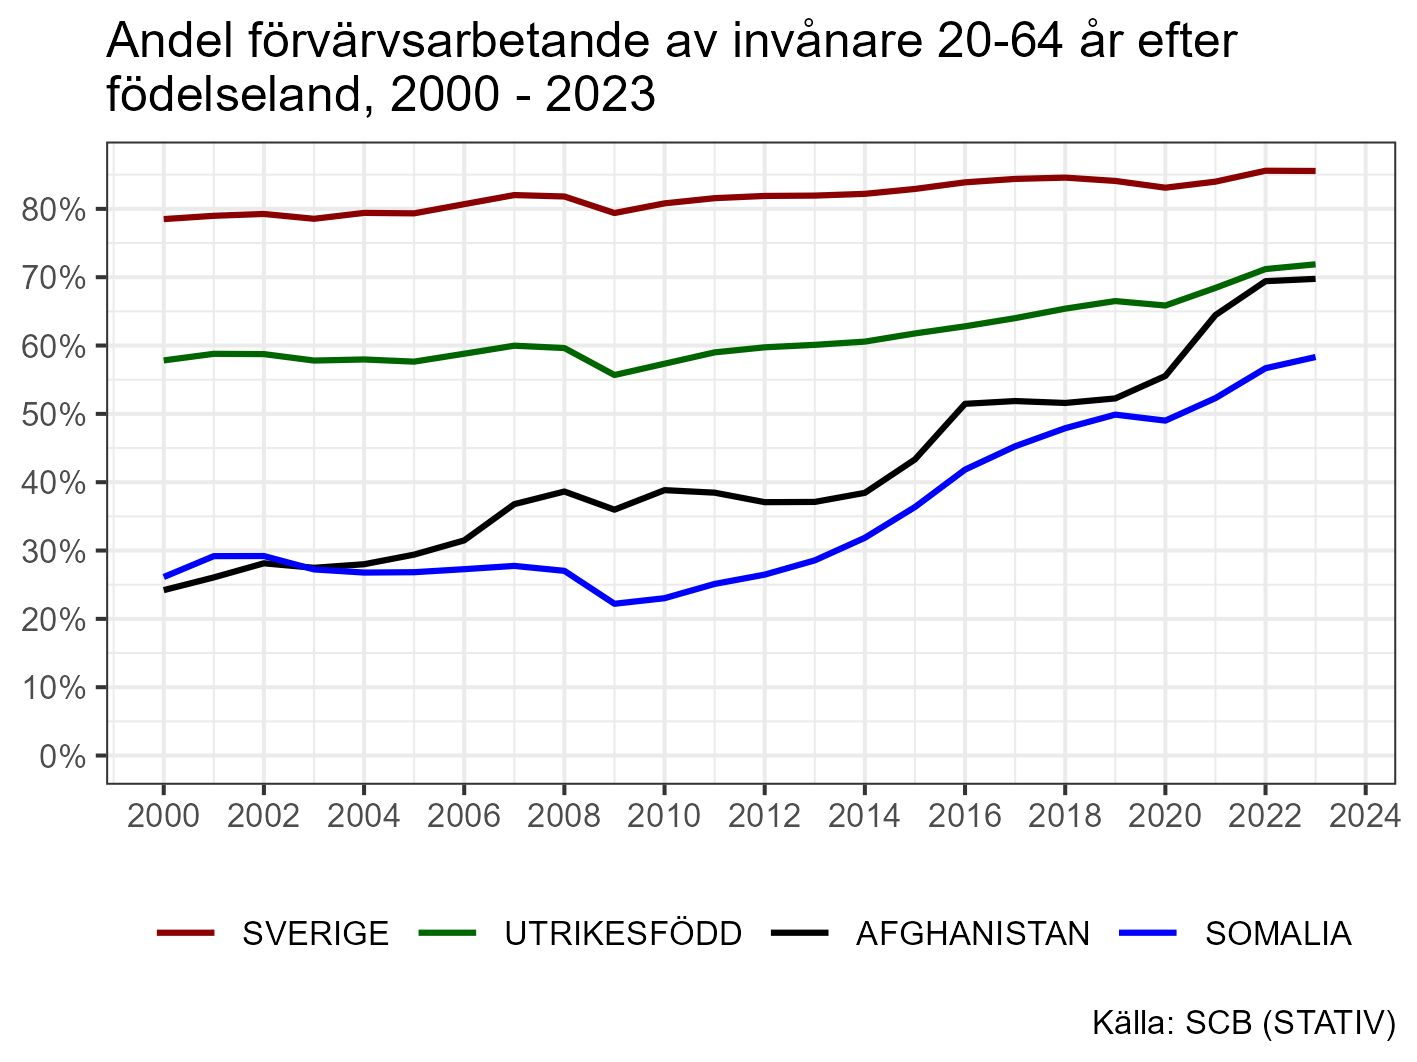
\includegraphics[width=6.20833in,height=\textheight,keepaspectratio]{bilder/sysgrad_fland/sys_fland_somalier_afgh.jpg}

\bookmarksetup{startatroot}

\chapter{Många deltidsarbetande kvinnor i EU-länderna jämfört med i
Sverige}\label{muxe5nga-deltidsarbetande-kvinnor-i-eu-luxe4nderna-juxe4mfuxf6rt-med-i-sverige}

Många kvinnor i EU-länderna arbetar deltid, vilket kan bero på olika
faktorer som familjeansvar, brist på heltidsjobb eller personliga
preferenser. I Sverige är det dock vanligare att kvinnor arbetar heltid
jämfört med många andra EU-länder. De länder som har hög andel
deltidsarbetande kvinnor inkluderar Nederländerna, Tyskland och
Österrike, där deltidsarbete är mer utbrett. I Sverige är det däremot
vanligare att kvinnor arbetar heltid, vilket kan bero på en mer
jämställd arbetsmarknad och bättre tillgång till barnomsorg.

Ett intressant undantag är att många av länderna i det forna östblocket,
som Polen, Tjeckien och Slovakien, har en hög andel kvinnor som arbetar
heltid. Detta kan bero på historiska och kulturella faktorer, där det
under kommunisttiden var vanligt att både män och kvinnor deltog i
arbetslivet, därtill kommer att det finns ekonomiska faktorer som gör
att kvinnor i dessa länder behöver arbeta heltid för att försörja sig
själva och sina familjer.

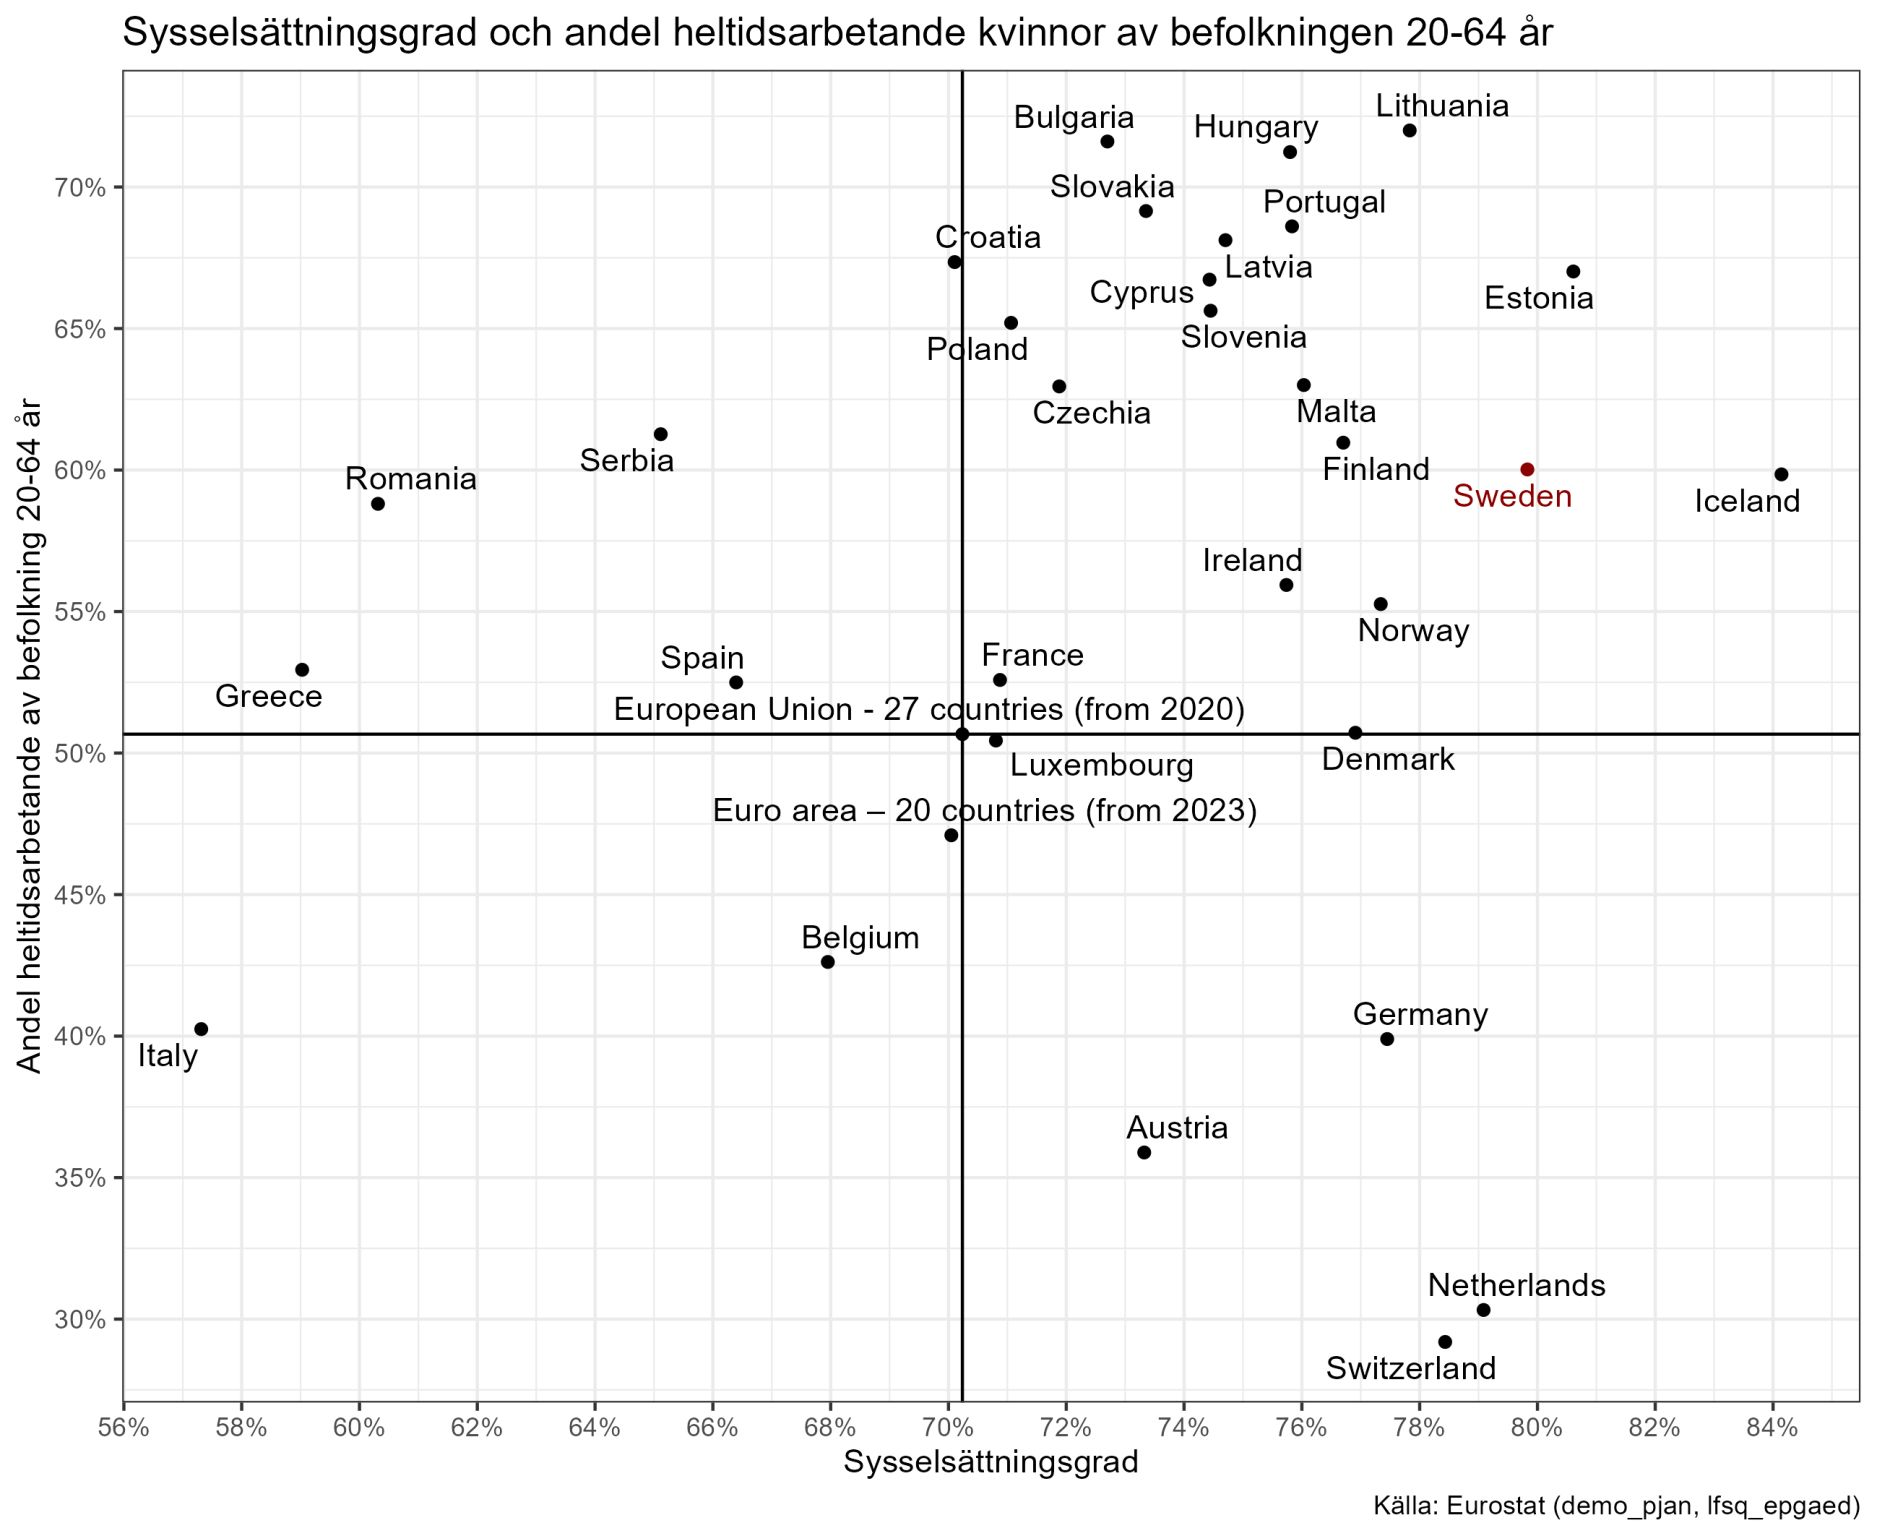
\includegraphics[width=7.86458in,height=\textheight,keepaspectratio]{bilder/heltid_deltid_kon_eu/sys_deltid_kon_eu.jpg}

\bookmarksetup{startatroot}

\chapter{Färre bidragsförsörjda och fler
utrikesfödda}\label{fuxe4rre-bidragsfuxf6rsuxf6rjda-och-fler-utrikesfuxf6dda}

Väldigt många tycks leva i villfarelsen att en allt högre andel av
befolkningen blir beroende av sociala ersättningar och bidrag i takt med
att andelen invandrare av befolkningen ökar. Men så är inte fallet.
Tvärtom är statistiken glasklar: Andelen ``bidragsförsörjda'' har
minskat i takt med att andelen utrikesfödda ökat.

Den stora flyktingvågen i mitten av 10-talet tycks inte haft någon
större inverkan på den sjunkande andelen av befolkningen som försörjs av
sociala ersättningar och bidrag. Tvärtom fortsatte den sjunkande
trenden.

Det finns sannolikt två förklaringar till den sjunkande andelen
``bidragstagande''. Den största förklaringen är troligen att en allt
högra andel av befolkningen förvärvsarbetar. Den andra förklaringen är
att det blivit svårare att kvalificera sig för att få tillgång till
samhällets skyddsnät. Om vi studerar utrikesfödda, vilka är kraftigt
överrepresenterade bland mottagare av ekonomisk bistånd kan vi se att
andelen förvärvsarbetande varit stigande under lång tid. De senaste
årens konjunkturnedgång har endast marginellt påverkat
sysselsättningsgraden för utrikesfödda. Enligt SCB:s preliminära
sysselsättningsstatistik (BAS) sjönk sysselsättningsgraden för
utrikesfödda med en halv procentenhet mellan februari 2024 och februari
2025, men steg sedan med 0,6 procentenheter mellan februari 2025 och
februari 2026.

\pandocbounded{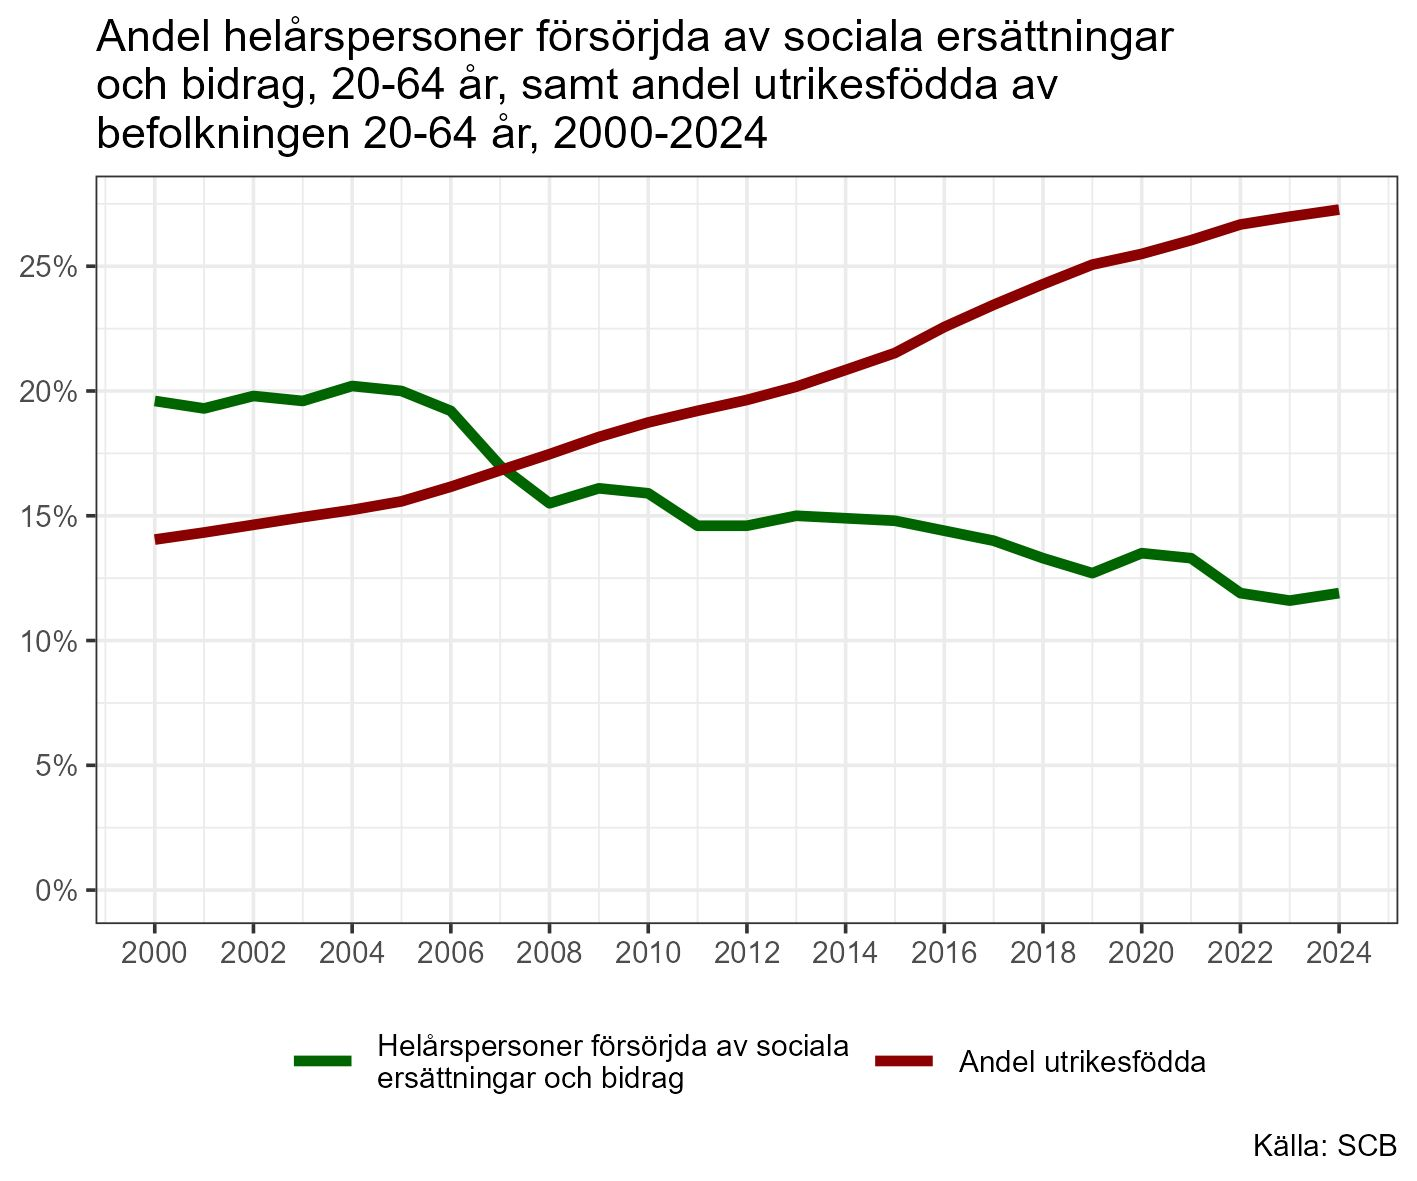
\includegraphics[keepaspectratio]{bilder/bidrag_och_utrikesfodda/bidrag_och_utrikesfodda.jpg}}

Källa:

\href{https://www.scb.se/hitta-statistik/statistik-efter-amne/hushallens-ekonomi/hushallens-inkomster-tillgangar-och-skulder/antalet-helarspersoner-som-forsorjdes-med-sociala-ersattningar-och-bidrag/pong/tabell-och-diagram/helarsekvivalenter/helarsekvivalenter-1990-2025/}{Sociala
ersättningar och bidrag 1990-2025 (excel)}

\bookmarksetup{startatroot}

\chapter{Rättelser}\label{ruxe4ttelser}

Trots att vi har försökt att vara noggranna så kan det finnas fel i
boken. Här samlar vi de fel som vi har hittat. Här har vi samlat
rättelser (eller \emph{errata} som det heter i finare sammanhang).

\bookmarksetup{startatroot}

\chapter*{References}\label{references}
\addcontentsline{toc}{chapter}{References}

\markboth{References}{References}

\protect\phantomsection\label{refs}




\end{document}
